% LeakLens paper draft.
% Compiles with pdflatex and a standard TeX Live (no venue class needed).
% To move to a venue template (IEEEtran, acmart, LNCS), keep the body from \section{Introduction}
% onwards and replace the preamble and the title block.
\documentclass[10pt,a4paper,twocolumn]{article}

\usepackage[T1]{fontenc}
\usepackage[utf8]{inputenc}
\usepackage{mathptmx}
\usepackage[scaled=0.9]{helvet}
\usepackage{courier}
\usepackage[a4paper,top=19mm,bottom=22mm,left=16mm,right=16mm,columnsep=6.5mm]{geometry}
\usepackage{microtype}
\usepackage{amsmath}
\usepackage{booktabs}
\usepackage{tabularx}
\usepackage{array}
\usepackage{multirow}
\usepackage{xcolor}
\usepackage{graphicx}
\usepackage{listings}
\usepackage{enumitem}
\usepackage{titlesec}
\usepackage{caption}
\usepackage{tikz}
\usetikzlibrary{arrows.meta,positioning}
\usepackage{pgfplots}
\pgfplotsset{compat=1.18}
\usepackage[hidelinks]{hyperref}
\usepackage{url}

\titleformat{\section}{\normalfont\large\bfseries}{\thesection.}{0.5em}{}
\titleformat{\subsection}{\normalfont\normalsize\bfseries}{\thesubsection}{0.5em}{}
\titlespacing*{\section}{0pt}{9pt plus 2pt minus 1pt}{4pt}
\titlespacing*{\subsection}{0pt}{7pt plus 2pt minus 1pt}{3pt}
\captionsetup{font=small,labelfont=bf,labelsep=period}
\setlist{nosep,leftmargin=1.3em}
\setlength{\parskip}{0pt}
\setlength{\parindent}{1em}
\renewcommand{\arraystretch}{1.12}
\definecolor{codebg}{HTML}{F5F6F8}
\definecolor{codegrey}{HTML}{5A626B}
\definecolor{navy}{HTML}{1F4E79}
\definecolor{sand}{HTML}{C9A66B}

\lstset{
  basicstyle=\ttfamily\scriptsize,
  backgroundcolor=\color{codebg},
  frame=single, rulecolor=\color{codebg},
  breaklines=true, columns=fullflexible, keepspaces=true,
  showstringspaces=false, xleftmargin=2pt, xrightmargin=2pt,
  aboveskip=5pt, belowskip=3pt,
  commentstyle=\color{codegrey}
}

\newcommand{\tool}{LeakLens}
\newcommand{\code}[1]{\texttt{#1}}

\begin{document}

\twocolumn[
\begin{center}
{\LARGE\bfseries LeakLens: Detecting Group and Temporal Data Leakage in Machine Learning Code by Linking Static Analysis to an Instrumented Run\par}
\vspace{11pt}
{\normalsize
\begin{tabular}{@{}c@{\hspace{9mm}}c@{\hspace{9mm}}c@{}}
\textbf{Srijeet Prasad Banerjee} & \textbf{Adrish Sarkar} & \textbf{Ankur Roy} \\[5pt]
\textbf{Sayandeep Dey} & \textbf{Soumyarik Mukherjee} & \textbf{Sayan Hazra} \\
\end{tabular}\par}
\vspace{7pt}
{\small Department of Information Technology, Guru Nanak Institute of Technology, Kolkata, India\par}
\vspace{12pt}
\begin{minipage}{0.90\textwidth}
\small
\noindent\textbf{Abstract.}
Data leakage lets information from the evaluation data reach model training, so a reported score no longer
predicts performance on new data. Tools that read machine learning code detect preprocessing, overlap and
multi-test leakage, but not group leakage (the same patient, user or device on both sides of a split), and they
cover temporal leakage only in part, although these are the kinds that distort results most. We present \tool{},
a prototype for Python scripts and notebooks. A static pass based on abstract interpretation reports six leakage
types and nominates the split call and the candidate entity or time column; an optional instrumented run checks,
fold by fold, whether entities or time periods overlap at that call, with nothing declared by the user; and a
located leak can be fixed in a copy of the pipeline and re-run to measure its effect on the pipeline's own metric.
On the held-out half of a benchmark of injected leaks (79 files, 73 leaks), scored once under a frozen protocol,
the static pass finds 59 leaks and the combined mode 65, with no false positive. Scored per file, the analyser of
Yang et al.\ is right for 20 of the 37 files with a leak of a type it supports, \tool{} for 33 ($p<0.001$). Given
the same exported splits, four data-level checkers and a run-time checker find group and time-order leaks only
once the right column is named; without it the best finds 3 of 8 shuffled time-series splits, \tool{} 8 of 8.
Only 3 of 7 group findings name the true entity, and a proxy-model tool estimated the impact of group leaks more
accurately. All results are on synthetic files written by the authors; real notebooks are not yet labelled.

\vspace{4pt}
\noindent\textbf{Keywords:} data leakage, static analysis, dynamic analysis, Jupyter notebooks, machine learning
engineering, reproducibility
\end{minipage}
\end{center}
\vspace{10pt}
]

\section{Introduction}

A machine learning score is meaningful only if the model never saw the evaluation data during training.
\emph{Data leakage} is any path by which evaluation rows, or information that is not available at prediction
time, influence training~\cite{kaufman2012}. Leaky code runs without error and its tests pass. The only symptom
is a score that is better than it should be.

Leakage is common. A survey of earlier reviews found it in 294 papers across 17 scientific fields; in one case
study, complex models lost their reported advantage over logistic regression once the errors were
corrected~\cite{kapoor2023}. A static analysis of 107,603 public GitHub notebooks reported at least one leak in
29.6\% of them~\cite{yang2022}.

Not all leaks do equal damage. Across 2,047 tabular datasets, fitting a scaler on all rows before splitting,
the textbook example, changed AUC by at most 0.005 in all nine conditions tested, while leakage across group and
time boundaries was invisible under random cross-validation~\cite{roth2026}. In translational EEG research, only
17 of 63 surveyed deep learning studies clearly avoided placing segments of one subject in both training and
test data, and in one experiment accuracy fell from 99.8\% to 53.0\% when subjects were held out
properly~\cite{brookshire2024}.

The tools that read code look mostly at the first kind. The reference static analyser of Yang et
al.~\cite{yang2022} and the tools built on it~\cite{alomar2025,truong2025,draoui2026} detect preprocessing,
overlap and multi-test leakage. To our knowledge, no published static analyser detects group leakage from source
code, and temporal leakage is covered in part by one recent LLM-based linter~\cite{samsonau2026}. Tools that
check the data itself can find date overlap~\cite{chorev2022} and group overlap~\cite{leakcheckml,leakhound}, but the user
has to export the training and test tables and usually name the column, and the result does not point to a line
of code. None of these tools reports how much a detected leak changes the user's own result.

This paper describes \tool{}\footnote{An unrelated package with the same name exists on PyPI. The name of
this project may change before any release.}, which addresses these three gaps. Its contributions are:

\begin{enumerate}
\item \textbf{Group leakage detected from source code}, with the entity inferred from column and variable names
and from identifiers derived from file paths. Temporal leakage is detected through data flow. This is not a
first for temporal leakage~\cite{samsonau2026}; we treat it as an improvement on existing code-level checks.
\item \textbf{A link from static findings to an instrumented run.} The static pass nominates the split call and
candidate columns; the run checks entity and time overlap at that call, per fold, with no user declaration.
\item \textbf{A per-finding impact estimate} obtained by re-running the user's own pipeline with a canonical fix.
\item \textbf{A benchmark of 175 files with 162 injected leaks} that includes group and temporal leakage, with a
development and test split fixed before any detection rule was written.
\end{enumerate}

Every number in this paper is measured on synthetic files that we generated; 150 real notebooks are sampled
but not yet labelled, so we make no claim about precision or recall on real code.

\section{Background and Related Work}

\textbf{Taxonomies.} Kaufman et al.~\cite{kaufman2012} gave the first formal treatment of leakage. Kapoor and
Narayanan~\cite{kapoor2023} describe eight types, among them preprocessing on training and test data together,
duplicates, temporal leakage and non-independence between training and test samples. Roth~\cite{roth2026}
measured severity by type in controlled experiments and found that the commonly taught type matters least.

\textbf{Static analysis of ML code.} Yang et al.~\cite{yang2022} model data flow in Datalog and report three
leakage types, with a precision of 97.6\% and a recall of 67.8\% on hand-labelled notebooks. NBLyzer and later
abstract-interpretation work verify the absence of contamination between training and test
data~\cite{subotic2022a,subotic2022b,drobnjakovic2024}. LeakageDetector wraps the analyser of Yang et al.\ in an
IDE and adds quick fixes~\cite{alomar2025,truong2025}. Draoui et al.~\cite{draoui2026} combine static slicing
with LLM prompts; their abstract reports F1 gains of 22\% for preprocessing and 15\% for overlap leakage over
earlier work (we could read only the abstract). scicode-lint~\cite{samsonau2026} asks a local LLM pattern
questions about scientific code; two of its patterns concern temporal leakage (shuffled cross-validation on
temporal data, and forward-looking shifts and centred windows). We found no group-leakage pattern among its
definitions.

\textbf{Checks on data and at run time.} Deepchecks~\cite{chorev2022} checks duplicate rows and date overlap between training and test tables supplied
by the user, and several recent packages add group overlap~\cite{leakcheckml,leakhound}. splitguard~\cite{splitguard} instruments splits and fits at run time and flags group
overlap at the split line, but only for group identifiers the user registers. ArgusEyes~\cite{schelter2023}
detects row overlap through provenance tracking in an instrumented run.

\textbf{Measuring the effect.} LeakHound~\cite{leakhound} estimates inflation with a proxy model that it trains
itself on the given split. mlwhatif~\cite{grafberger2023} re-executes user pipelines with patches, for
data-cleaning questions rather than leakage. Leakly~\cite{leakly} re-runs a whole pipeline on permuted labels;
a score above chance suggests leakage somewhere, without locating it or applying a fix. \tool{} differs in that
the estimate belongs to one located finding and is measured on the user's own pipeline and metric.

Table~\ref{tab:design} compares \tool{} with the analyser of Yang et al., the closest prior work and the engine
inside the LeakageDetector tools.

\begin{table*}[t]
\caption{Design comparison between the static analyser of Yang et al.\ and \tool{}. Entries for Yang et al.\
are taken from their paper and from our own runs of their released tool. The two accuracy rows were measured on
different data with different labelling and are not comparable; Table~\ref{tab:yang} gives the only like-for-like
measurement.}
\label{tab:design}
\footnotesize
% Table 1 (rebuilt 2026-11-13 from the draft PDF; entries checked in docs/COMPARISON_TABLE_CHECK.md).
% 2026-11-14: rows Input, Confidence/severity, Output, Dependencies and Large-scale study removed for space;
% group row and accuracy row updated (strict entity rule, EVAL_CHANGES #10; hand-written splits, #13).
\begin{tabularx}{\textwidth}{@{}>{\raggedright\arraybackslash}p{0.17\textwidth}>{\raggedright\arraybackslash}X>{\raggedright\arraybackslash}X@{}}
\toprule
\textbf{Aspect} & \textbf{Yang et al.~\cite{yang2022}} & \textbf{\tool{} (this work)} \\
\midrule
Analysis technique & Static data-flow analysis written in Datalog (Souffl\'{e}), with type inference & One-pass abstract interpretation over the Python syntax tree, linked to an optional instrumented run \\
Runs the analysed code & No & Optional (dynamic and impact modes only) \\
Leakage types & Preprocessing, overlap, multi-test & The same three, plus group, temporal and target-derived features \\
Group and temporal leakage & Not types it claims & Group: entity from column names, file paths, attributes of items, or a column found at run time; confirmed at the split. Temporal: non-chronological splits, forward-looking features \\
Location reported & The affected evaluation line (as observed in our runs) & The line that causes the leak, with a suggested fix \\
Impact on the score & Not estimated & Re-runs the pipeline with a canonical fix (six kinds); preliminary \\
Evaluation data & 100 hand-labelled real notebooks (94 analysed) and 107,603 public GitHub notebooks & 175 synthetic files with injected leaks; five real-code case studies; 79 real notebooks being labelled \\
Accuracy reported by the authors & Precision 97.6\% (40/41), recall 67.8\% (40/59), real notebooks & Recall 0.81 (static, no false positive) and 0.84 (with the run, 4 false positives), own injected TEST split, correct entity required \\
Time per file & Mean 3.23\,s (their paper); median 6.2\,s on our files (Kaggle CPU) & Static: median 2.6\,ms. Instrumented run: median 1.3\,s (laptop) \\
\bottomrule
\end{tabularx}

\end{table*}

\section{Leakage Taxonomy}

\tool{} reports six types (Table~\ref{tab:types}). The first three correspond to the types of Yang et
al.~\cite{yang2022}. Group and temporal leakage correspond to non-independence and temporal leakage in the
taxonomy of Kapoor and Narayanan~\cite{kapoor2023}, and target-derived features to their illegitimate features.

\begin{table}[t]
\caption{The six leakage types and the signal used by each pass.}
\label{tab:types}
\footnotesize
\begin{tabularx}{\columnwidth}{@{}>{\raggedright\arraybackslash}p{0.19\columnwidth}>{\raggedright\arraybackslash}X>{\raggedright\arraybackslash}X@{}}
\toprule
\textbf{Type} & \textbf{Static signal} & \textbf{Run-time check} \\
\midrule
Preprocessing & A transformer, selector or encoder is fitted on rows that later reach the evaluation side & The fit included evaluation rows \\
Overlap & Resampling or concatenation before the split; evaluation rows flow into a fit & Identical rows on both sides of the split \\
Multi-test & Several candidates scored on the same evaluation rows feed a selection & Same rows scored repeatedly \\
Group & A row-level splitter or default CV on data with a candidate entity & The same entity value on both sides \\
Temporal & A shuffled split on time-ordered data; forward-looking feature & Training rows dated after evaluation rows \\
Target-derived & A feature computed from the label & Very high single-feature score \\
\bottomrule
\end{tabularx}
\end{table}

A group finding depends on the claim being made. A model meant to be used on the same patients it was trained
on may legitimately share patients across a split. The tool cannot know the claim, so group findings carry a
confidence level and can be suppressed inline with a stated reason.

\section{Design of LeakLens}

Figure~\ref{fig:pipeline} shows the three stages. The static stage never runs the analysed code. The other two
execute it and are optional.

\begin{figure}[t]
\centering
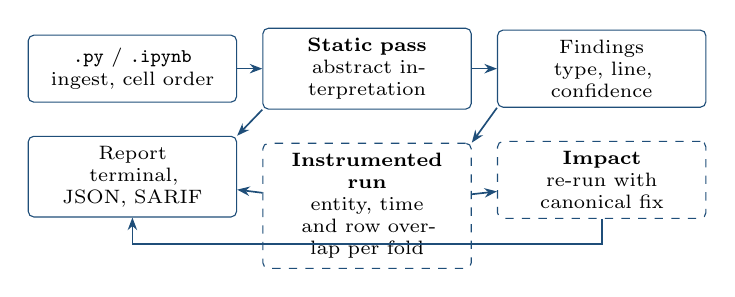
\begin{tikzpicture}[
  node distance=4.2mm and 3.2mm,
  box/.style={draw=navy, rounded corners=2pt, align=center, font=\scriptsize, inner sep=3.5pt, minimum height=8.5mm, text width=24mm, fill=white},
  opt/.style={box, dashed},
  arr/.style={-{Stealth[length=1.6mm]}, navy, semithick}]
\node[box] (in) {\code{.py} / \code{.ipynb}\\ingest, cell order};
\node[box, right=of in] (st) {\textbf{Static pass}\\abstract interpretation};
\node[box, right=of st] (fi) {Findings\\type, line, confidence};
\node[opt, below=of st] (dy) {\textbf{Instrumented run}\\entity, time and row overlap per fold};
\node[opt, below=of fi] (im) {\textbf{Impact}\\re-run with canonical fix};
\node[box, below=of in] (re) {Report\\terminal, JSON, SARIF};
\draw[arr] (in) -- (st);
\draw[arr] (st) -- (fi);
\draw[arr] (fi.south west) -- (dy.north east);
\draw[arr] (dy) -- (im);
\draw[arr] (dy) -- (re);
\draw[arr] (st.south west) -- (re.north east);
\draw[arr] (im.south) -- ++(0,-3.2mm) -| (re.south);
\end{tikzpicture}
\caption{Stages of \tool{}. Dashed stages execute the code and are optional.}
\label{fig:pipeline}
\end{figure}

\subsection{Static pass}

Notebooks are read in execution order when every code cell has a unique execution count, and in cell order
otherwise. The analyser then makes one pass of abstract interpretation over the flattened module. Each variable
receives an abstract value that records what the analysis knows: the origin of a data frame, its known columns,
which statistics have been computed over which rows, whether rows have been copied or resampled, and the
training or evaluation role of the result of a split.

Rules fire at \emph{sinks}. At a split point (\code{train\_test\_split}, a splitter's \code{split}, a
cross-validation helper, a search object, or a manual random sample with its complement) the analyser checks for
group and temporal leakage and reports every statistic or copied row that reached the data being split. At a
model fit it reports statistics computed on rows that include the evaluation side. At a prediction or score it
checks whether the model was fitted on rows that include the scored rows. A selection over scores computed in a
loop gives a multi-test finding.

For group leakage, the evidence for an entity is a column or variable name, or an identifier derived from a file
path (for example a subject code split from a recording's file name). Names are matched against two lists.
Strong names such as \code{patient}, \code{subject} or \code{user} can give a finding of medium confidence. Weak
names such as \code{customer}, \code{id} or \code{visit} give low confidence only. Listing~\ref{lst:example}
shows a file-path case.

\begin{lstlisting}[float=t, caption={Group leakage through cross-validation with the default splitter, and the finding the static pass reports for the full file (code and message shortened).}, label={lst:example}, captionpos=b]
recordings = {f"sub-{i:02d}_run-1.npy": ... }
windows, labels, subjects = [], [], []
for fname, signal in recordings.items():
    subject = fname.split("_")[0]
    for w in signal.reshape(-1, 500):
        windows.append([w.mean(), w.std()])
        labels.append(...)
        subjects.append(subject)
X, y = np.array(windows), np.array(labels)
print(cross_val_score(LogisticRegression(), X, y, cv=5).mean())

line 16  [high/medium] group (LL-GRP-003)
  Rows are split without regard to `subjects`; the same
  subjects can be in training and evaluation rows.
  fix: use GroupKFold with groups=`subjects`
\end{lstlisting}

The analyser prefers missing a leak to inventing one. A call it does not model is treated as depending on all its
inputs, and anything it cannot resolve produces no finding. Loops are analysed once, functions are inlined to a
fixed depth, and classes are opaque. pandas, NumPy, scikit-learn~\cite{sklearn} and imbalanced-learn are
modelled by name; all catalogues and thresholds are in configuration files.

\subsection{Instrumented run}

Static analysis cannot see an entity column that the code never mentions. A script may load a table with a
\code{patient\_id} column and split it at random without naming that column. The dynamic pass handles this
case. It runs the script in a child process with scikit-learn entry points wrapped: \code{train\_test\_split},
the \code{split} method of every splitter, the cross-validation helpers, estimator \code{fit}, \code{predict}
and \code{score}, and the metric functions.

At each split, and for each fold, the wrapper records three facts. Rows are hashed by value, after rounding
numbers, to find identical rows on both sides. Entity columns are looked up in the data frames of the script's
own namespace that are row-aligned with the data being split; a column is reported when its values repeat and
enough evaluation rows belong to an entity that also has training rows. If a time column is found, the wrapper
checks whether training rows are dated after the earliest evaluation row.

These facts are linked to the static findings by call site. A finding ends up \emph{confirmed}, \emph{refuted}
or \emph{not checked} (no run-time check exists for that rule). Findings that only the run can make, such as
duplicate records already present in the raw data, are added.

\subsection{Impact estimation}

For a located finding, \tool{} re-runs the script with one call site changed and nothing else. Six kinds of fix
are implemented: duplicated records are removed before a split; a row-level split becomes a group-aware one on
the detected column; a non-chronological split becomes a chronological one; evaluation rows are removed from a
model fit; a transformer fitted on all rows is fitted on the training rows of a hold-out split; and a feature is
removed. The estimate is the script's printed metric in the original run minus the metric in the fixed run.
Findings without an automatic fix, or whose fixed run fails, are reported as ``impact unknown'' and are never
dropped. When the fixed run takes a different path through the code, the estimate is marked unreliable.

\subsection{Running untrusted code}

The dynamic and impact modes execute the analysed file. For notebooks from the internet, \tool{} runs them only
through a sandbox inside an offline cloud session: a child process with an allow-listed environment, a
throwaway working directory, a process-group timeout and an unprivileged user. Each layer answers a problem we
measured. The platform we use (Kaggle) injects session tokens into every job, and a child process running as root could
read them from \code{/proc} even with a clean environment. After the privilege drop, a scan from the child
found the token in none of its ancestor processes, while a control scan as root found it in two.

\subsection{Reporting and integration}

Each finding carries the file, line range, type, rule identifier, confidence, severity, evidence, a suggested
fix and, when measured, the metric before and after the fix. Output formats are terminal text, JSON with a
published schema, and SARIF, which GitHub code scanning accepts. A pre-commit hook and a GitHub Action are
provided. The tool is deterministic and uses no language model. Its test suite has 373 tests, including
property-based tests that the analyser terminates and gives identical output on repeated runs; on a laptop 371
pass and the 2 sandbox tests that need root are skipped (they pass as root in the cloud job).

\section{Benchmark and Evaluation Protocol}

\subsection{Injected benchmark}

No public labelled dataset includes group and temporal leakage, so we built one. Thirteen clean base pipelines
in three families (tabular, time series and grouped data such as multi-visit patients and EEG-style windows) are
mutated by 18 operators. Seventeen inject a leak, for example a scaler fitted before the split, oversampling
before the split, a shuffled split on time-ordered data, or a row-level split on grouped data. One produces a
\emph{trap}: code that resembles a leak but is correct. Six files combine two leaks. The result is 175 files (94
scripts and 81 notebooks) with 162 labelled leaks, 13 clean files and 6 traps. The lines that carry each leak
are known by construction, and every leaky file has a corrected version, so the true inflation of its metric
can be measured.

Temporal leaks are divided into three categories: \emph{common} (for example an explicit shuffled split),
\emph{differentiating} (cases that pattern-based checks do not cover, such as the default shuffle of
\code{train\_test\_split}) and \emph{hard} (for example a time column with a name that does not suggest time).

The benchmark is split by base pipeline into DEV (7 pipelines, 96 files, 89 leaks) and TEST (6 pipelines, 79
files, 73 leaks). The assignment was committed before any detection rule existed. Rules and thresholds were
tuned on DEV only.

\subsection{Real notebooks}

We sampled 150 public Kaggle notebooks in three query-based strata of 50 and split them by author into DEV (71)
and TEST (79), to be labelled by two people who see no tool output, with Cohen's kappa reported. \textbf{This
labelling has not been done.} On the 71 DEV notebooks the static pass ran without a crash (median 4\,ms per
notebook); without labels, what it flagged is not a result.

\subsection{Protocol}

The protocol was written after DEV results had been seen and frozen before any TEST result existed. A finding
matches a label when it is in the same file and cell, its lines overlap the labelled lines, and its type is the
labelled type or a listed alternative; matching is one-to-one, an unmatched finding is a false positive and an
unmatched label a miss. The operating point is medium or higher confidence. Recall is reported per type with 95\%
percentile bootstrap intervals over files (2,000 resamples). TEST is scored once per release; any later change is
logged and its result labelled a second look. The true inflation of an injected file is the metric of the leaky
file minus that of its corrected version, averaged over five data seeds. The generators were designed, and for
group leakage adjusted after a first measurement, so that each leak type can change the metric; these values
therefore score detection and impact estimates only and are no evidence of severity in practice.

\subsection{Baselines}

\textbf{Yang et al.} We built the released analyser~\cite{yang2022} from source in a Linux cloud job and ran its
default command. Its packaged Datalog engine no longer installs, so the engine was built at version 2.4.1, a
deviation from the released setup; notebooks were given as plain scripts, as its documentation requires. It
reports the affected evaluation line, not the leaking line, so both tools are scored per file and type: a tool is
right about a type in a file when it reports that type and the file has a labelled leak of that type. This rule
was fixed before any baseline output on TEST existed.

\textbf{Data-level and run-time tools.} leakcheck-ml~\cite{leakcheckml}, LeakHound~\cite{leakhound},
dataleaks~\cite{dataleaks} and Deepchecks~\cite{chorev2022} take a training and a test table, not code. The
instrumented run of \tool{} exports, at every split call and for up to five folds, the tables the pipeline used
(every row-aligned column of the script's data frames, the label column removed and the target kept apart). Each
tool received every pair twice, with its defaults and with the true entity or time column named through its own
parameter; a detection is placed at the split call's line. splitguard~\cite{splitguard} instruments a run itself
and was run as documented, and again with the true group declared through \code{mark\_groups}. Each tool ran in its
own environment at the cited version (Deepchecks needs Python 3.11 and NumPy~1.26). For every tool a finding is one
per file, line and type. These untuned tools ran in jobs after the single TEST run of \tool{}.

\textbf{Not run.} scicode-lint~\cite{samsonau2026} needs a GPU with at least 16\,GB and native FP8 support. On two
NVIDIA T4 GPUs (no FP8) its pinned server (vLLM~0.18.0) failed to start, and a fallback (llama.cpp, same model at
8 bits) produced no result within 20 minutes for any of the 29 files it attempted; it is reported as not run, not
as zero. LeakCheck~\cite{draoui2026} needs a paid LLM interface and an access-restricted package.

\section{Results}

\subsection{Detection on the held-out split}

Table~\ref{tab:test} gives the single TEST run: 59 of 73 leaks found statically (0.81) and 65 with the run (0.89),
no false positive in either mode, and no finding on the 9 leak-free files. The run confirmed 43 static findings,
refuted none, could not check 25 (no run-time check exists for forward-looking features or pandas statistics) and
added 2, both duplicated records. By temporal category the tool found 5 of 5 common, 7 of 7 differentiating and 8
of 13 hard leaks. On DEV, where the rules were tuned, it found 80 of 89 statically and 89 of 89 with the run; the
drop from DEV to TEST is real.

\begin{table}[t]
\caption{Detection on the injected TEST split (79 files, 73 leaks), scored once. Findings of medium or higher
confidence. Recall with 95\% bootstrap interval over files. No false positive in either mode.}
\label{tab:test}
\footnotesize
\setlength{\tabcolsep}{3.2pt}
\begin{tabular}{@{}lrrlrl@{}}
\toprule
 & & \multicolumn{2}{c}{\textbf{Static}} & \multicolumn{2}{c}{\textbf{Static + run}} \\
\cmidrule(lr){3-4}\cmidrule(l){5-6}
\textbf{Type} & \textbf{Leaks} & \textbf{Found} & \textbf{Recall} & \textbf{Found} & \textbf{Recall} \\
\midrule
Preprocessing & 22 & 21 & 0.95 (0.84--1.00) & 21 & 0.95 (0.84--1.00) \\
Overlap & 9 & 7 & 0.78 (0.44--1.00) & 9 & 1.00 (1.00--1.00) \\
Multi-test & 6 & 5 & 0.83 (0.43--1.00) & 5 & 0.83 (0.43--1.00) \\
Group & 7 & 3 & 0.43 (0.00--0.83) & 7$^{*}$ & 1.00$^{*}$ \\
Temporal & 25 & 20 & 0.80 (0.62--0.95) & 20 & 0.80 (0.62--0.95) \\
Target-derived & 4 & 3 & 0.75 (0.00--1.00) & 3 & 0.75 (0.00--1.00) \\
\midrule
All types & 73 & 59 & 0.81 & 65 & 0.89 \\
\bottomrule
\end{tabular}

\vspace{2pt}
\raggedright $^{*}$By the matching rule, which checks type and line. Only 3 of the 7 findings name the true
entity column, so the strict figure is 0.43.
\end{table}

\subsection{What went wrong on TEST, and a second look}

\textbf{Right line, wrong column.} In a patient-visits pipeline the static pass made a low-confidence guess on a
column named \code{visit}; the confirmation step looked only at nominated columns, found visit numbers on both
sides of the split, as they always are, and raised the confidence without examining \code{patient\_id}. The
matching rule does not check the column, so Table~\ref{tab:test} counts these four findings as correct. They are
not, and neither is the impact estimate that follows. \textbf{A slice mistaken for a split.} A pipeline dropping
its last row with \code{data.iloc[:-1]} was read as the training side of a manual split: five temporal leaks
were reported at low confidence only and one multi-test leak was missed. \textbf{An unresolved column filter.} A
feature list built with a \code{startswith} filter could not be resolved, so two leaks were not reported.

The three faults were then fixed and logged. DEV was re-run unchanged, and TEST again gave 67 of 73 with the
static pass and 73 of 73 with the run, with no false positive; the patient findings now name \code{patient\_id},
and the EEG ones a run-time variable holding the subject identifiers. The fixes were written knowing which TEST
files they repair, so this is not a held-out result and Table~\ref{tab:test} remains the result of record. The
injected benchmark is now saturated on both halves.

\subsection{Comparison with Yang et al.\ on the same files}

On the three types the baseline supports (Table~\ref{tab:yang}), it found 20 of 37 files with one false alarm, and
the static pass of \tool{} 33 of 37 with none; both analysed all 79 files and reported nothing on the leak-free
ones. On the 37 file-and-type pairs \tool{} alone was right in 14, the baseline alone in 1, both in 19 and neither
in 3 (exact McNemar test, $p=0.001$). The difference comes from preprocessing (12 against 1); on overlap the tools
agree on every file. The comparison favours \tool{}: neither tool was tuned on these files, but they were
generated by our operators, with the kinds of leak \tool{} was built for. The figures the baseline's authors
report on their own notebooks (precision 97.6\%, recall 67.8\%) are a different measurement and cannot be set
against Table~\ref{tab:yang}.

\begin{table}[t]
\caption{Yang et al.\ and \tool{} (static mode) on the 79 injected TEST files, scored per file and type.
``Found'': files with this leak in which the tool reports the type. ``False'': files where it reports the type
wrongly.}
\label{tab:yang}
\footnotesize
\setlength{\tabcolsep}{4.5pt}
\begin{tabular}{@{}lrrrrr@{}}
\toprule
 & & \multicolumn{2}{c}{\textbf{Yang et al.~\cite{yang2022}}} & \multicolumn{2}{c}{\textbf{\tool{} (static)}} \\
\cmidrule(lr){3-4}\cmidrule(l){5-6}
\textbf{Leakage type} & \textbf{Files} & \textbf{Found} & \textbf{False} & \textbf{Found} & \textbf{False} \\
\midrule
Preprocessing & 22 & 10 & 1 & 21 & 0 \\
Overlap / duplicates & 9 & 7 & 0 & 7 & 0 \\
Multi-test & 6 & 3 & 0 & 5 & 0 \\
\midrule
Group$^{\dagger}$ & 7 & 0 & 0 & 3 & 0 \\
Temporal$^{\dagger}$ & 24 & 3 & 0 & 19 & 0 \\
Target-derived$^{\dagger}$ & 4 & 0 & 0 & 3 & 0 \\
\bottomrule
\end{tabular}


\vspace{2pt}
\raggedright $^{\dagger}$Not a type the baseline claims to detect. It is credited under temporal in 3 files where
it reports whole-series scaling as preprocessing leakage. Temporal has 24 files for 25 leaks because one file
holds two.
\end{table}

\subsection{Leaks at a split: data-level and run-time tools}

Table~\ref{tab:baselines} covers the TEST leaks at a split call, the only ones a data-level tool can see: 8
non-chronological splits of time-ordered data, 7 group splits and 2 sets of duplicated raw records. Without a
named column, leakcheck-ml finds 4 of 7 group splits, all with the right column, and 3 of 8 time splits;
LeakHound, Deepchecks and splitguard find none of either. With the column named, leakcheck-ml and LeakHound find
7 of 8 and 7 of 7. dataleaks reaches 7 of 7 group splits without a hint, but names an unrelated column in 3 and
reports a group overlap in 2 of the 9 leak-free files; its default configuration has no split-order check.
Deepchecks has no group check and finds time splits only when told the time column. splitguard finds group
splits only when the group is declared, and does not see the held-out rows of a split taken with
\code{next(splitter.split(...))}. All data-level tools find the duplicated records.

\tool{} finds 8 of 8 time splits without being told any column. On group splits it is weaker than the rule-based
count suggests: only 3 of its 7 findings name the true entity, against 4 for leakcheck-ml without a hint. Every
other tool also needs the user to export the tables, which the instrumented run of \tool{} did for them here.

\begin{table}[t]
\caption{Leaks at a split call, injected TEST. Col.: whether the true entity or time column was named to the
tool. T1: non-chronological splits of time-ordered data. Grp: group splits by the matching rule; Grp, col.: group
findings that name the true entity column. Dup.: duplicated raw records. Clean: leak-free files with any finding.
\tool{}: first look, result of record.}
\label{tab:baselines}
\footnotesize
\setlength{\tabcolsep}{2.6pt}
\begin{tabular}{@{}llrrrrr@{}}
\toprule
\textbf{Tool} & \textbf{Column given} & \textbf{T1} & \textbf{Grp} & \textbf{Grp, col.} & \textbf{Dup.} & \textbf{Clean} \\
 & & /8 & /7 & /7 & /2 & /9 \\
\midrule
\tool{} (static + run) & none needed & 8 & 7 & 3 & 2 & 0 \\
\midrule
leakcheck-ml & none (default) & 3 & 4 & 4 & 2 & 0 \\
 & true column named & 7 & 7 & 7 & 2 & 0 \\
leakhound-ml & none (default) & 0 & 0 & 0 & 2 & 0 \\
 & true column named & 7 & 7 & 7 & 2 & 0 \\
dataleaks & none (default) & 0 & 7 & 4 & 2 & 2 \\
 & true column named & 0 & 7 & 7 & 2 & 2 \\
deepchecks & none (default) & 0 & 0 & 0 & 2 & 0 \\
 & true column named & 7 & 0 & 0 & 2 & 0 \\
splitguard & none (default) & 0 & 0 & 0 & 0 & 0 \\
 & true column named & 0 & 7 & 7 & 0 & 0 \\
\bottomrule
\end{tabular}

\end{table}

\subsection{Impact estimates}

On TEST an estimate could be produced for 34 of 70 located leaks (group 7 of 7, target-derived 3 of 3, overlap 7
of 9, preprocessing 10 of 21, temporal 7 of 25, multi-test 0 of 5); the rest are reported as unknown with the
reason. The instrumented script printed exactly the plain script's metric in all 395 runs. For 26 single-leak
findings with a bounded metric, averaged over five seeds, the mean absolute error against the true inflation was
0.035 and the rank correlation 0.58. The estimate was exact where our fix is the same operation as the
benchmark's corrected file, a weak test, and wrong in direction for hold-out group splits ($-0.084$ against a
true $+0.212$ AUC) because the fix grouped by the wrong column. In the second look the error was 0.0006 and the
correlation 0.97, with the same caveat as for detection.

LeakHound (Table~\ref{tab:impact}) trains its own model on the exported split and compares it with a group-aware
or chronological split it builds; it reports AUC or $R^2$, so only pipelines with those metrics are compared, on
seed 0. Where both tools gave an estimate (11 findings), LeakHound's mean absolute error was 0.065 and \tool{}'s
0.086: \tool{} was worse on the hold-out group splits, where it grouped by the wrong column, and exact on
duplicated records and time splits, where LeakHound was off by 0.01 to 0.08. With the column fault repaired
(second look, not held out) \tool{}'s error on the same 11 findings was 0.020. LeakHound gave no estimate for
preprocessing or target-derived findings, and none without a named column except for duplicated records. The
near-zero preprocessing errors carry little information, as the true inflation of those leaks is close to zero.

\begin{table}[t]
\caption{Impact estimates against the true inflation, injected TEST, single-leak files, seed 0. N: findings.
Comp.: findings whose pipeline reports AUC or $R^2$, the metrics LeakHound reports. Cells: number of estimates
(mean absolute error). LH: LeakHound with its defaults; LH, col.: with the true column named. \tool{}: first
look.}
\label{tab:impact}
\footnotesize
\setlength{\tabcolsep}{2.4pt}
\begin{tabular}{@{}lrrlll@{}}
\toprule
\textbf{Type} & \textbf{N} & \textbf{Comp.} & \textbf{\tool{}} & \textbf{LH} & \textbf{LH, col.} \\
\midrule
group & 6 & 6 & 6 (0.158) & 0 (--) & 6 (0.075) \\
overlap & 6 & 6 & 6 (0.000) & 2 (0.043) & 2 (0.043) \\
preproc. & 8 & 8 & 8 (0.000) & 0 (--) & 0 (--) \\
target-der. & 3 & 3 & 3 (0.000) & 0 (--) & 0 (--) \\
temporal & 6 & 3 & 3 (0.000) & 0 (--) & 3 (0.059) \\
\bottomrule
\end{tabular}

\end{table}

\subsection{Running time and a negative case study}

The static pass took a median of 2.6\,ms per file and the instrumented run 1.3\,s (maximum 12.7\,s) on a laptop;
the Yang analyser took a median of 6.2\,s per file in a cloud CPU job. The machines differ, so these figures
indicate scale only.

We also ran the static pass on a separate EEG seizure-detection codebase by the first author, with three
evaluation regimes of known leakage status: random windows, a within-patient split and leave-one-patient-out. The
tool reported nothing in its 78 files: correct for the third regime, a miss for the first two. The code splits
with hand-written NumPy masks and by position over lists of custom objects, and subject identity is an object
attribute; there is no scikit-learn splitter, data frame or column name to model, and the dynamic pass would not
see these splits either. No rule was changed after this result.

\section{Limitations and Threats to Validity}

\textbf{No result on real code.} All figures come from our own injected benchmark; the tool and the benchmark
share authors, and TEST uses different pipelines but the same mutation operators as DEV. The results measure
generalisation across pipelines, not across the ways people write leaks, and a precision of 1.00 on short
synthetic files will not hold on real notebooks. \textbf{Small samples.} TEST has 4 target-derived, 6 multi-test
and 7 group leaks; the intervals are wide. \textbf{Blindness.} The column names of the TEST pipelines were seen by
mistake while rules were written; no TEST code, label or operator was read, but TEST group results are not blind
to entity names. \textbf{Heuristic entity inference.} Evidence for an entity is a name, repetition or a file path;
a name can mislead in both directions, as the first TEST run shows. \textbf{Coverage of code styles.} pandas,
NumPy and scikit-learn are modelled by name; hand-written splits, custom classes and deep learning frameworks are
largely outside the analysis, as the case study shows. \textbf{Impact estimates.} Automatic fixes exist for six
situations, about half of the located leaks; a group-aware or chronological split changes which rows are
evaluated, so an estimate is the change under the canonical fix, not a causal decomposition.
\textbf{Baselines.} The Yang analyser was scored under a looser rule than the protocol's; the data-level tools
were given tables exported by our instrumented run and ran after the single TEST run of \tool{}; scicode-lint and
LeakCheck could not be run.

\section{Conclusion and Future Work}

\tool{} detects six types of data leakage in Python machine learning code, including group leakage from source
code, links static findings to facts observed in an instrumented run, and estimates the effect of a located leak
by re-running the pipeline with a fix. On held-out injected leaks it found 81\% of leaks statically and 89\% with
the run, with no false positive, and more leaks than the reference static analyser on the three types they share
($p=0.001$). Against data-level tools given the same splits it was the only tool to find the time-order leaks
without being told the time column, and it was matched or beaten on group leaks by a tool told the entity column.
The evaluation also exposed a confirmation fault that named the wrong entity in four of seven group findings, and
a case study on real code showed that hand-written splits are invisible to it.

The next step decides whether these results hold outside our benchmark: labelling the 150 sampled notebooks and
scoring \tool{} and the baselines on them. We then plan to run scicode-lint on hardware with FP8 support, to extend
the analysis to manual and framework-specific splits, and to measure how often each leakage type occurs in public
notebooks and how much it changes their reported scores.

\section*{Data and Code Availability}

The source code, benchmark generators, frozen protocol, evaluation change log and the output of every run cited
here are in the project repository: \url{https://github.com/bytes06runner/LeakLens}.

\section*{Acknowledgement}

The implementation was written with the help of an AI coding assistant. The authors made the design and
protocol decisions and reviewed the results reported here.

\begin{thebibliography}{99}
\scriptsize
\setlength{\itemsep}{0.5pt}

\bibitem{kaufman2012} S. Kaufman, S. Rosset, C. Perlich, and O. Stitelman, ``Leakage in data mining: formulation,
detection, and avoidance,'' \emph{ACM Trans. Knowl. Discov. Data}, vol. 6, no. 4, 2012.
doi:10.1145/2382577.2382579.

\bibitem{kapoor2023} S. Kapoor and A. Narayanan, ``Leakage and the reproducibility crisis in
machine-learning-based science,'' \emph{Patterns}, vol. 4, no. 9, 100804, 2023. doi:10.1016/j.patter.2023.100804.

\bibitem{yang2022} C. Yang, R. A. Brower-Sinning, G. A. Lewis, and C. K\"{a}stner, ``Data leakage in notebooks:
static detection and better processes,'' in \emph{Proc. 37th IEEE/ACM Int. Conf. Automated Software Engineering
(ASE)}, 2022. doi:10.1145/3551349.3556918.

\bibitem{roth2026} S. Roth, ``Which leakage types matter? A quantitative landscape across 2,047 benchmark
datasets,'' arXiv:2604.04199, 2026.

\bibitem{brookshire2024} G. Brookshire \emph{et al.}, ``Data leakage in deep learning studies of translational
EEG,'' \emph{Front. Neurosci.}, vol. 18, 1373515, 2024. doi:10.3389/fnins.2024.1373515.

\bibitem{alomar2025} E. A. AlOmar, C. DeMario, R. Shagawat, and B. Kreiser, ``LeakageDetector: an open source
data leakage analysis tool in machine learning pipelines,'' arXiv:2503.14723, 2025.

\bibitem{truong2025} Truong \emph{et al.}, ``LeakageDetector 2.0: analyzing data leakage in Jupyter-driven
machine learning pipelines,'' arXiv:2509.15971, 2025.

\bibitem{draoui2026} T. Draoui, M. W. Mkaouer, and C. Newman, ``Improving data leakage detection in machine
learning notebooks through static slicing and structured LLM prompts,'' \emph{Proc. ACM Softw. Eng.}, vol. 3,
no. FSE, 2026. doi:10.1145/3808199.

\bibitem{samsonau2026} Samsonau, ``scicode-lint: detecting methodology bugs in scientific Python code with
LLM-generated patterns,'' arXiv:2603.17893, 2026.

\bibitem{subotic2022a} P. Suboti\'{c}, L. Miliki\'{c}, and M. Stoji\'{c}, ``A static analysis framework for data
science notebooks,'' in \emph{Proc. 44th Int. Conf. Software Engineering: Software Engineering in Practice
(ICSE-SEIP)}, 2022. doi:10.1145/3510457.3513032.

\bibitem{subotic2022b} P. Suboti\'{c}, U. Bojani\'{c}, and M. Stoji\'{c}, ``Statically detecting data leakages in
data science code,'' in \emph{Proc. 11th ACM SIGPLAN Int. Workshop on the State of the Art in Program Analysis
(SOAP)}, 2022. doi:10.1145/3520313.3534657.

\bibitem{drobnjakovic2024} F. Drobnjakovi\'{c}, P. Suboti\'{c}, and C. Urban, ``An abstract interpretation-based
data leakage static analysis,'' in \emph{Theoretical Aspects of Software Engineering (TASE)}, LNCS, Springer,
2024. doi:10.1007/978-3-031-64626-3\_7.

\bibitem{chorev2022} S. Chorev \emph{et al.}, ``Deepchecks: a library for testing and validating machine learning
models and data,'' \emph{J. Mach. Learn. Res.}, vol. 23, no. 285, 2022.

\bibitem{schelter2023} S. Schelter, S. Grafberger, S. Guha, B. Karla\v{s}, and C. Zhang, ``Proactively screening
machine learning pipelines with ArgusEyes,'' in \emph{Companion of the 2023 Int. Conf. Management of Data
(SIGMOD)}, 2023. doi:10.1145/3555041.3589682.

\bibitem{grafberger2023} S. Grafberger, P. Groth, and S. Schelter, ``Automating and optimizing data-centric
what-if analyses on native machine learning pipelines,'' \emph{Proc. ACM Manag. Data (SIGMOD)}, 2023.
doi:10.1145/3589273.

\bibitem{sklearn} F. Pedregosa \emph{et al.}, ``Scikit-learn: machine learning in Python,'' \emph{J. Mach.
Learn. Res.}, vol. 12, pp. 2825--2830, 2011.

\bibitem{splitguard} T. Aiello, ``splitguard,'' software, version 0.1.0, 2026.
\url{https://github.com/Tommasoaiello13/splitguard}.

\bibitem{leakhound} J. Gomes, ``LeakHound,'' software, version 0.5.0, 2026.
\url{https://github.com/happyhellpt/leakhound}.

\bibitem{leakcheckml} ``leakcheck-ml,'' software, version 0.3.0, 2026.
\url{https://github.com/Sofienguy1/leakcheck}.

\bibitem{dataleaks} K. Rajput, ``DataLeaks,'' software, version 0.1.2, 2026.
\url{https://github.com/KAVYA-29-ai/Dataleaks}.

\bibitem{leakly} DeMONLab-BioFINDER, ``Leakly: leakage checks for machine-learning pipelines using permutation tests,''
software, version 0.1.2, 2026. \url{https://github.com/DeMONLab-BioFINDER/Leakly}.

\end{thebibliography}

\end{document}
